\chapter{Customizing Tao}
\index{customizing}
\label{c:custom.tao}

%----------------------------------------------------------------
\section{It's all a matter of Hooks}
\index{customizing!hooks}

The golden rule when extending \tao is that you are only allowed to
replace routines or redefine structures that have the name ``hook'' in
them.  If you have the source code then it's within your power to
modify any routine in \tao as much as you like. However, as time goes
by, and revisions are made to the \tao routines to extend the
usefulness of \tao and to eliminate bugs, only modifying the ``hook''
routines will ensure that custom changes will have a minimum impact on
the specialized routines that will be written by various people.

\tao is written in Fortran 95 and a knowledge of Fortran is
required. However, if you know C then Fortran can be learned in a
couple of days. Because of the interoperability between C and Fortran
once the wrapper routines are written to interface with \tao the rest
of your coding can, in principle all be done in C.

\tao relies on extensive use of pointers and logical flags. However,
all of the structures you will need to use are contained in the
\vn{tao_struct.f90} module. This module is heavily documented and
provides all the information needed to use the intrinsic \tao
structures on your customizations. It is also a very good idea to have
a copy of \vn{bmad_struct.f90} handy as this contains most of the
structures used by \bmad.

%----------------------------------------------------------------
\section{Compiling your custom Tao}
\index{customizing!compiling}

The \tao libraries can be compiled without compiling an
executable. Here is where this comes in handy. Since the standard \tao
subroutines have already been made into libraries, all you need to do
is compile and link your custom routines with the standard \tao
subroutines into an executable.

There are 11 ``hook'' files located in the \cmd{ROOT/tao/hook}
directory. These are the files you can customize. There are two
options here.
\begin{enumerate}
  \item Change the files directly in \cmd{ROOT/tao/hook}, adding any extra
    files you may need, then recompile from the \cmd{ROOT/tao} directory with
  \cmd{gmake -f M.tao}.  \label{cust.option.one}
  \item Copy the hook files to a separate directory say \cmd{ROOT/my_tao},
    adding any extra files you may need, then write a Makefile to 
    compile and link these
    routines to the main \tao library. \label{cust.option.two}
\end{enumerate}
Option~\ref{cust.option.two} is HIGHLY recommended because it keeps
the \tao distribution tree undisturbed and reserves the possibility to
create multiple custom \tao programs using the same vanilla \tao
library. This option is used in the following example.

%----------------------------------------------------------------
\section{An Example}
\index{customizing!example}

As an example let's include a new data type called
\vn{particle_emittance}. This will be the non-normalized x and y
emittance as found from the Courant-Snyder invariant. This data type
will behave just like any other data type (i.e.  \vn{orbit},
\vn{phase} etc...). First, we should copy all the hook files to a
separate directory, call it \cmd{ROOT/my_tao}. Also include the main
program file from the \cmd{ROOT/tao/program} directory.  (replace
\vn{ROOT} with whatever top directory you placed the \vn{tao}
directory.)
\begin{example}
  mkdir ROOT/my_tao
  cp ROOT/tao/hook/*.f90 ROOT/my_tao
  cp ROOT/tao/program/tao_cl.f90 ROOT/my_tao/my_tao_cl.f90
\end{example}
Next we need a Makefile. The \cmd{ROOT/tao/M.tao} 
Makefile is a great starting point.
\begin{example}
  cp ROOT/tao/M.tao ROOT/my_tao/Makefile
\end{example}
Now change the following lines in your Makefile
\begin{example}
  LIB_SRC_DIRS := ./code ./hook
  OBJ_SRC_DIRS := ./program
\end{example}
to
\begin{example}
  LIB_SRC_DIRS :=
  OBJ_SRC_DIRS := ./
\end{example}
This Makefile will tell gmake to use the tao library that has already
been created (from \cmd{../tao/code} but the actual library is located
at \cmd{../lib/libtao.a})
 and then to compile
all of the hook files, including the main program file
(\cmd{my_tao_cl.f90}) into object files (everything in \cmd{./}, the
current directory).  Routines and declarations in object files always
override similarly named code in the \tao libraries so this allows for
your local hook files to override the dummy hook files in the \tao
library. The only downside to this method is it clutters your
\cmd{my_tao} directory with object files. You can always remove these
object files with \cmd{gmake clean}.

There are two more lines to alter. change
\begin{example}
  MAIN_FILE :=
\end{example}
to
\begin{example}
  MAIN_FILE := ./my_tao_cl.f90
\end{example}
and finally,
\begin{example}
  MAKEFILE := M.tao
\end{example}
to
\begin{example}
  #MAKEFILE := M.tao !using default name for Makefile
\end{example}
Notice that this line is just being commented out with a `\#'. You are
now ready to make your customizations to the hook routines.

This example will only require the modification of one file:
\vn{tao_hook_evaluate_a_datum.f90}. The formula for single particle
emittance is
\Begineq
  \epsilon = \gamma x^{2} + 2 \alpha x x' + \beta x'^{2}
  \label{e:emittance}
\Endeq
Place the following code in \vn{tao_hook_evaluate_a_datum.f90} in the
\cmd{case select} construct (also add the necessary type declarations)
\begin{verbatim}
  case ('particle_emittance.x') 

    datum_value =  ( ele%x%gamma * tao_lat%orb(ix1)%vec(1)**2 + &
		     2 * ele%x%alpha * tao_lat%orb(ix1)%vec(1) * tao_lat%orb(ix1)%vec(2) + &
		     ele%x%beta * tao_lat%orb(ix1)%vec(2)**2)
    
  case ('particle_emittance.y')

    datum_value = ( ele%y%gamma * tao_lat%orb(ix1)%vec(3)**2 + &
		     2 * ele%y%alpha * tao_lat%orb(ix1)%vec(3) * tao_lat%orb(ix1)%vec(4) + &
		     ele%y%beta * tao_lat%orb(ix1)%vec(4)**2)
\end{verbatim}
This defines what is to be calculated for each \vn{particle_emittance}
datum.  There are two transverse coordinates, so two definitions need
to be made, one for each dimension.

Now you just need to declare the data types in the \cmd{tao.init} and
\cmd{tao_plot.init} files. For the sake of this example, modify the
initialization files used for this tutorial.
\begin{example}
  cp ROOT/tao/program/*.init ROOT/my_tao
  cp ROOT/tao/program/*.lat ROOT/my_tao
\end{example}

In \cmd{ROOT/my_tao/tao.init} add the following lines to the data
declarations section
\begin{example}
  &tao_d2_data
    d2_data%name = "particle_emittance" 
    universe = 0 
    n_d1_data = 2
  /

  &tao_d1_data
    ix_d1_data = 1
    d1_data%name = "x"  
    default_weight = 1
    use_same_lat_eles_as = 'orbit.x"
  /

  &tao_d1_data
    ix_d1_data = 2
    d1_data%name = "y"  
    default_weight = 1
    use_same_lat_eles_as = 'orbit.x"
  /
\end{example}

In \cmd{ROOT/my_tao/tao_plot.init} add the following lines to the end
of the file
\begin{example}
  &tao_template_plot
    plot%name = 'particle_emittance'
    plot%x%min =   0
    plot%x%max = 100
    plot%x%major_div = 10
    plot%x%label = ' '
    plot%x_axis_type = 'index'
    plot%n_graph = 2
  /
  
  &tao_template_graph
    graph%name = 'x'
    graph_index = 1
    graph%box = 1, 2, 1, 2
    graph%title = 'Horizontal Emittance (microns)'
    graph%margin =  0.15, 0.06, 0.12, 0.12, '%BOX'
    graph%y%label = 'x'
    graph%y%max =  15
    graph%y%min =  0.0
    graph%y%major_div = 4
    graph%n_curve = 1
    curve(1)%data_source = 'dat'
    curve(1)%data_type   = 'particle_emittance.x'
    curve(1)%y_axis_scale_factor = 1e6 !convert from meters to microns
  /

  &tao_template_graph
    graph%name = 'y'
    graph_index = 2
    graph%box = 1, 1, 1, 2
    graph%title = 'Vertical Emittance (microns)'
    graph%margin =  0.15, 0.06, 0.12, 0.12, '%BOX'
    graph%y%label = 'Y'
    graph%y%max =  15
    graph%y%min =  0.0
    graph%y%major_div = 4
    graph%n_curve = 1
    curve(1)%data_source = 'dat'
    curve(1)%data_type = 'particle_emittance.y'
    curve(1)%units_factor = 1e6 !convert from meters to microns
  /
\end{example}
These namelists are described in detail in Chapter~\ref{c:init}.

We are now ready to compile and then run the program. The \tao library
should have already been created so all you need to do is
\begin{example}
  cd ROOT/my_tao
  gmake
  ../bin/my_tao
\end{example}
Notice that the name of the custom \tao program is \cmd{my_tao}. If you run 
`\cmd{../bin/tao}' then you will run ``vanilla'' \tao.

After your custom \tao initializes type
\begin{example}
  place bottom particle_emittance
  scale
\end{example}
Your plot should look like Figure~\ref{f:plot.emittance}.

The emittance (as calculated) is not constant. This is due to
dispersion and coupling throughout the ring. \bmad provides a routine
to find the particle emittance from the twiss parameters that includes
dispersion and coupling called \vn{orbit_amplitude_calc}.

\begin{figure}
  \centering
  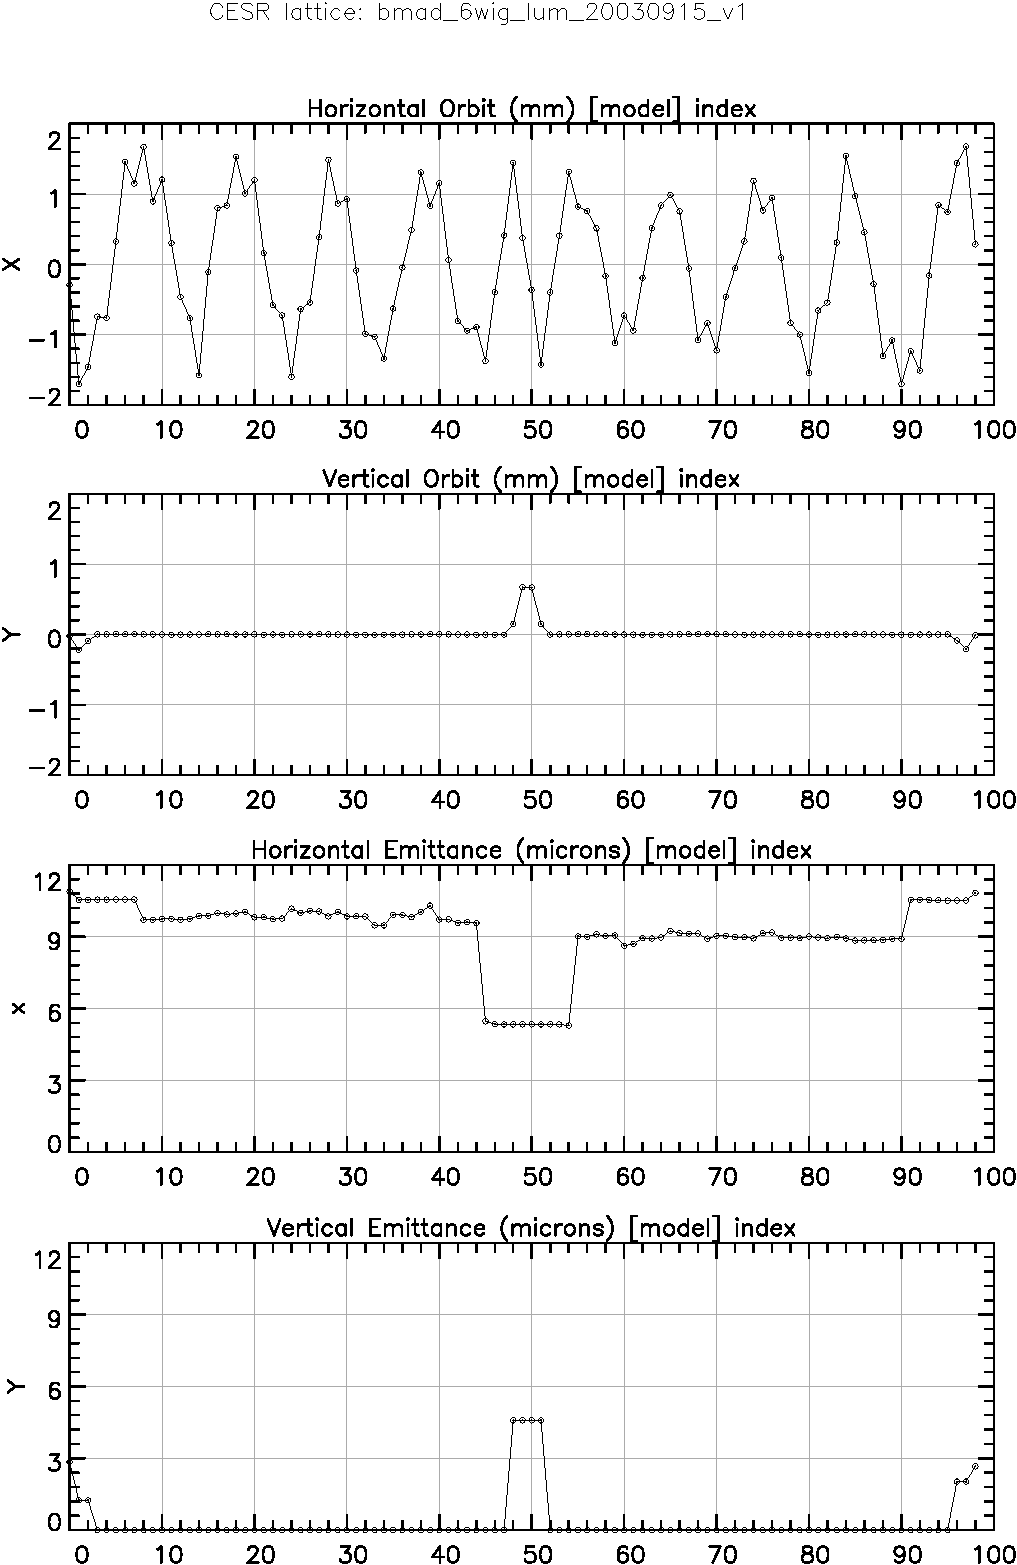
\includegraphics[width=5in]{plot-emittance.pdf}
  \caption{Custom data type: non-normalized emittance}
  \label{f:plot.emittance}
\end{figure}

\Section{Other Customizations}

The above example just illustrates one of the customizations you can
perform on \tao. The next chapter lays out all of the
hook files and provides pointers for various customizations.

